\documentclass{llncs}

\usepackage{makeidx}
\usepackage{xspace}
\usepackage[dvips]{graphicx}
\usepackage{adjustbox}
\usepackage{graphicx}
\usepackage{blindtext}
\usepackage{algorithm}
\usepackage{cite}
\usepackage[noend]{algpseudocode}
\usepackage{multirow}
\usepackage{mathtools}
\usepackage{mathrsfs}
\usepackage{multicol}
\usepackage{enumitem}
\usepackage{extarrows}
\usepackage{caption}
\usepackage{subcaption}
\usepackage{amsmath, amsfonts, amssymb}
\usepackage{bbm}
\usepackage{stmaryrd}
\usepackage{mathtools}
\usepackage[mathscr]{eucal}
\usepackage{bm}
\usepackage{array}
\usepackage{url}
\usepackage{calc}
\usepackage{float}
\usepackage{latexsym}
\usepackage{multirow}
\usepackage{subcaption}
\usepackage{fmtcount}
\DeclareGraphicsExtensions{.eps,.jpg,.png,.pdf}
\usepackage[usenames, dvipsnames, table]{xcolor}
\usepackage{todonotes}
\usepackage[bookmarks,bookmarksdepth=2]{hyperref}
\hypersetup{colorlinks,linkcolor=black,urlcolor=blue}
\usepackage{multicol}
\usepackage{siunitx}
\usepackage{enumitem}
\usepackage{comment}
\usepackage{dashrule}
\usepackage{environ}
\usepackage{xargs}
\usepackage{hhline}
\usepackage{tikz}
\usepackage{circuitikz}
\usepackage{tikz-timing}[2009/12/09]
\usepackage{pgfplots}
\usetikzlibrary{shapes.geometric}
\usepackage{booktabs}
\usepackage{fixme}
\fxsetup{status=draft, nomargin, inline}
\fxusetheme{color}
\renewcommand{\algorithmicrequire}{\textbf{Input:}}
\renewcommand{\algorithmicensure}{\textbf{Output:}}

\newcommand\raisepunct[1]{\,\mathpunct{\raisebox{0.5ex}{#1}}}
\tikzset{latency/.style={path picture={ 
    \draw[black]
  (-.4, .1) -- (-0.1, 0.25) (-.4,.4) -- (-.1, 0.25);
  \draw[black]
  (-.4, .1) -- (-0.1, -0.05) (-.4,.-.2) -- (-.1, -0.05);
  }}}
  \tikzset{latencysbox/.style={path picture={ 
    \draw[black]
  (.3, -.5) -- (.45, -.2) (.45,-.2) -- (.6, -.5);
  }}}
\tikzset{mux 4by2/.style={muxdemux,
muxdemux def={Lh=4, NL=4, Rh=3,
NB=1, w=1, square pins=1}}}

\tikzset{mux 3by2/.style={muxdemux,
muxdemux def={Lh=4, NL=3, Rh=3,
NB=1, w=1, square pins=1}}}

\tikzset{mux 2by2/.style={muxdemux,
muxdemux def={Lh=3, NL=2, Rh=2,
NB=1, w=1, square pins=1}}}
\newcommand{\register}[1]{ node[rectangle, draw, minimum height = .75cm, minimum width = .75cm, name={#1}, bottomreg] {}}
\newcommand{\registerrot}[1]{ node[rectangle, draw, minimum height = .75cm, minimum width = .75cm, name={#1}, leftreg] {}}
\newcommand{\registerEn}[1]{ node[rectangle, draw, minimum height = .75cm, minimum width = .75cm, name={#1}, enable] {}}
\newcommand{\ro}[1]{ node[name={#1}, rectangle, rounded corners=3pt, minimum width=.5cm, minimum height=.8cm, draw, sparsam] {$\rho$}}
\newcommand{\rospa}[1]{ node[name={#1}, rectangle, fill = SPAgreen, rounded corners=3pt, minimum width=.5cm, minimum height=.8cm, draw, sparsam] {$\rho$}}
\newcommand{\rodpa}[1]{ node[name={#1}, fill = DPAblue, rectangle, rounded corners=3pt, minimum width=.5cm, minimum height=.8cm, draw, sparsam] {$\rho$}}
\newcommand{\tencdpa}[1]{ node[minimum size=1.25cm, fill = DPAblue, rounded corners=1ex, draw, name={#1}] {$\mathsf{\tilde{E}_{K, N}}$}}

\newcommand{\xor}[1]{ node[circle, inner sep=-1.3pt, name={#1}] {$\oplus$}}
\tikzset{bottomreg/.style={path picture={ 
  \draw[black]
(path picture bounding box.south west) -- (path picture bounding box.center) (path picture bounding box.south east) -- (path picture bounding box.center);
}}}
\tikzset{enable/.style={path picture={ 
  \node[] at (0,.25) {\footnotesize en};
    \draw[black]
(path picture bounding box.south west) -- (path picture bounding box.center) (path picture bounding box.south east) -- (path picture bounding box.center);
}}}
\tikzset{leftreg/.style={path picture={ 
  \draw[black]
(path picture bounding box.south west) -- (path picture bounding box.center) (path picture bounding box.north west) -- (path picture bounding box.center);
}}}
\newcommand{\xord}[1]{node [draw,circle,addition,minimum width=.4 cm, name = {#1}] {}}
\tikzset{addition/.style={path picture={ 
    \draw[black]
  (path picture bounding box.south) -- (path picture bounding box.north) (path picture bounding box.west) -- (path picture bounding box.east);
  }}}
  
\newcommand{\bitwidth}{\tikz{\draw[-] (-2pt,-2pt) -- (2pt, 2pt);}}

\tikzset{bitwidth/.style={above=-1pt, font=\tiny}}
\tikzset{bitwidthvert/.style={right = -1pt, font=\tiny}}
\usetikzlibrary{arrows, shapes.gates.logic.US, calc}
\tikzset{
  contact/.style={
    circle, 
    fill=black,
    minimum size=5pt, 
    inner sep=0pt,
    anchor=center,
  },
}
\newcommand{\andd}[1]{node [draw,circle,cross,minimum width=.4 cm, thick, name = {#1}] {}}
\tikzset{next/.style={->, >=latex}}
\tikzset{cross/.style={path picture={ 
    \draw[black]
  (path picture bounding box.south east) -- (path picture bounding box.north west) (path picture bounding box.south west) -- (path picture bounding box.north east);
  }}}
\tikzset{addition/.style={path picture={ 
    \draw[black]
  (path picture bounding box.south) -- (path picture bounding box.north) (path picture bounding box.west) -- (path picture bounding box.east);
  }}}
% color definition
\definecolor{SPAvgreen}{RGB}{0,154,23}
\definecolor{SPAgreen}{RGB}{127,255,0}
\definecolor{DPAblue}{RGB}{0,64,255}

\newcommand{\rate}{.5cm}
\newcommand{\perm}[1]{ node[rectangle, rounded corners=3pt, minimum width=.5cm, minimum height=1.8cm, draw, sparsam] {$\pi^{#1}$}}
\newcommand{\boxele}[1] {node [rectangle, rounded corners=3pt, minimum width=1.5cm, minimum height=1.2cm, draw, sparsam, thick, name = {#1}] {$\mathtt{#1}$}}
\newcommand{\permspa}[1]{ node[rectangle, fill = SPAgreen, rounded corners=3pt, minimum width=.5cm, minimum height=1.8cm, draw, sparsam] {$\pi^{#1}$}}
\newcommand{\permdpa}[1]{ node[rectangle, fill = DPAblue, rounded corners=3pt, minimum width=.5cm, minimum height=1.8cm, draw, sparsam] {$\pi^{#1}$}}
\newcommand{\permspav}[1]{ node[rectangle, fill = SPAvgreen, rounded corners=3pt, minimum width=.5cm, minimum height=1.8cm, draw, sparsam] {$\pi^{#1}$}}
\tikzset{sparsam/.style={inner sep=1pt}}
\newcommand{\xorspa}[1]{ node[circle, fill = SPAgreen, inner sep=-1.3pt, name={#1}] {$\oplus$}}
\newcommand{\xorspav}[1]{ node[circle, fill = SPAvgreen, inner sep=-1.3pt, name={#1}] {$\oplus$}}
\newcommand{\msg}{.7cm}
\newcommand{\minnext}{.4cm}
\newcommand{\phase}{1.7cm}
\newcommand{\xordpa}[1]{ node[circle, fill = DPAblue, inner sep=-1.3pt, name={#1}] {$\oplus$}}

\newcommand{\tbc}[1]{ node[minimum size=1.25cm,rounded corners=1ex, draw, name={#1}] {$\mathsf{\tilde{E}}$}}
\newcommand{\tbcdpa}[1]{ node[fill = DPAblue, minimum size=1.25cm,rounded corners=1ex, draw, name={#1}] {$\mathsf{\tilde{E}}$}}
\newcommand{\tbcspa}[1]{ node[fill = SPAgreen, minimum size=1.25cm,rounded corners=1ex, draw, name={#1}] {$\mathsf{\tilde{E}}$}}
\newcommand{\tbcspav}[1]{ node[fill = SPAvgreen, minimum size=1.25cm,rounded corners=1ex, draw, name={#1}] {$\mathsf{\tilde{E}}$}}

\newcommand{\skinnyll}{\ensuremath{S_{\mathrm{LL}}}\xspace}
\newcommand{\skinnyb}{\ensuremath{S_{\mathrm{B}}}\xspace}
\newcommand{\skinnys}{\ensuremath{S_{\mathrm{S}}}\xspace}
\newcommand{\asconp}{\ensuremath{\text{Ascon-p}}\xspace}

\newcommand{\randtake}{\overset{\$}{\gets}}
\renewcommand{\vec}[1]{\mathbf{#1}}
\newcommand{\sharing}[2][]{\vec{{#2}}^{#1}}
\newcommand{\gf}[1]{\mathbb{F}_{#1}}
\newcommand{\ft}{\gf{2}}
\newcommand{\reg}{\textsf{Reg}}
\newcommand{\func}[2]{#1\left(#2\right)}
\newcommand{\nShares}{d}
\newcommand{\algrule}[1][.2pt]{\par\vskip.5\baselineskip\hrule height #1\par\vskip.5\baselineskip}
\newcommand{\share}[3][]{\sharing[#1]{#2}_{#3}}

\newcommand{\algorithmautorefname}{Algorithm}
\def\sectionautorefname{Section} 
\def\subsectionautorefname{Section} 
\def\appendixautorefname{Appendix}


\begin{document} 

\title{Side-Channel Analysis of Kyber's	Arithmetic Encodings: a Cautionary Note}
%\author{Corentin Verhamme\inst{1} \and Ga\"{e}tan Cassiers\inst{1,2,3} \and Fran\c{c}ois-Xavier Standaert\inst{1}}
%\institute{ICTEAM, Universit\'{e} catholique de Louvain, Louvain-la-Neuve, Belgium \and TU Graz, Graz, Austria \and Lamarr Security Research, Graz, Austria}
%----------------------------------------------------------------
\maketitle

\begin{abstract}

\end{abstract}


\section{Introduction}

\todo{1.PKE to PQC}
PKE schemes are threatening under quantum computing. This thread leads to the need for new cryptographical schemes that are secure even if the adversary has sufficient quantum power. In 07/2023, Kyber was officially selected as the standard post-quantum cryptographical scheme by NIST. The security of Kyber is based on the hardness of solving the learning-with-errors problem in module lattices(MLWE problem [66]).

\todo{SCA on KYBER}
Despite the concrete CPA-secure for public key encryption (PKE) and CCA-secure for key encapsulation mechanism (KEM), Kyber has been proven to be vulnerable under various Side-channel Attacks (SCA), from SPA in \fxwarning{citation} to DPA in \fxwarning{citation}. Therefore, many publications were dedicated to improving side-channel resilience for Kyber's implementation. The most prominent countermeasure used is masking with several optimizations.\todo{Add brief SCA into}
Masking for Kyber differs from masking for former symmetric or asymmetric key schemes since the computations happen in binary and prime fields and the special distribution of the secret. Even though it can use ready tools available for both cases, Boolean masking for the first field and arithmetic masking for the latter. Both masking schemes have been carefully studied and yielded very concrete, provable security levels \fxwarning{cite Provable proof for Boolean masking and arithmetic masking}.
\todo{Masking}

However, constraints over these concrete results do not allow a direct induction to arithmetic masking for Kyber since the coefficients of the secret polynomials have centered binomial distribution on relatively small support.
Therefore, in this note, we, for the first time, take a closer look at arithmetic masking, specifically for Kyber, and provide a distinct angle of how different the scheme is compared to former well-studied encodings, thus motivating a deeper look at the subject.\todo{add relevant citations }
\todo{maybe split it to subsection? Masking proofs, arithmetic noise amplification, ...}

We first give several notions and notations needed for the note in Section \ref{sec:bg}. Next, an analysis on simulated data is carried in Section \ref{sec:sim} and finally, a quick evaluation proceeded on real measurements in Section \ref{sec:onm} aims to verify the relevance of former results.
\section{Background}\label{sec:bg}
We now recall some necessary notations and notions for the rest of the paper.
\subsection*{Crystal-Kyber}
\subsubsection*{Polynomial Arithmetic}
Kyber computations work on polynomial ring $R_q = \mathbb{Z}_q[X]/(X^n + 1)$ where $q$ is a prime that allow efficient Number Theory Transformation and $n$ is the size of message space. 
The polynomials are denoted as lower case $f \in R_q$ and have the form:
\begin{equation}
	f = f_0 + f_1\cdot X^1 + \dots + f_{n-1}\cdot X^{n-1}
\end{equation}
where each coefficient $f_i$ lies in one residue class in $\mathbb{Z}_q$.
The secret $\mathbf{s}$ in Kyber is a vector of $k$ polynomials in $R^k_q$ such that each polynomial $\mathbf{s}[i] \in R_q$.
\todo{Mention PKE, KEM Encaps Decaps?}
\subsubsection*{Centered binomial distribution}

For the sake of simplicity we use upper cases to denote random variables and calligraphic letters to denote sets.
A random variable $X$ we denote $X \overset{\$}{\leftarrow} \mathcal{X}$ where $X$ is uniform distributed over $\mathcal{X}$ and $X \leftarrow D$ when $X$ is chosen according to the distribution $D$.\\
Noise in Kyber is sampled from centered binomial distribution $\beta_{eta}$ for $\eta=2$ or $\eta=3$ and is defined as:
$$
s \leftarrow \beta_{\eta}
(a_1, a_2, \dots, a_{\eta}, b_1, b_2, \dots, b_{\eta}) \overset{\$}{\leftarrow} \{0, 1\}^{2\eta}
s = \sum_{i=1}^{\eta}(a_i-b_i)
$$
The parameters set of Kyber for Round 3 of the NIST competition is summarized in below table:\todo{Add spec table}
Since this note focus on encoding of polynomials we take $n, q, \eta$ value as in the table but keep $k=1$ for simplicity of the analysis.

Several SCA were proven to be threatening to the prime arithmetic computations in KYBER.Decaps \fxwarning[]{citations}, thus, countermeasures required on the process to project the scheme. Furthermore, few of them especially exploit the fact that the noise (i.e. the secret also) of KYBER lies in a small range of the field \fxwarning[]{citations}. Countermeasures applied to this part of the computation therefore, is somehow irregular \fxnote[]{wording} 



\subsubsection*{Sharing Encoding}


Masking is a popular countermeasure against DPA that aims to randomizing the intermediate values that are processed by the device thus making the side-channel leakage independent of the sensitive values. It generally works for most of the cryptographic schemes and has been extensively studied, even got provable security. The core idea of masking is to probabilistically split the sensitive variables into $d$ shares, the cryptographic computations process on shares and only combined at the end to get the correct output. If the information of any $d-1$ tuple of shares reveals nothing about the sensitive value then $d$-share masking (i.e. $d+1$ masking) was proven to be secure against $d+1$-order SCA.\fxwarning{Double check and add citation}

In a $d$-share masked implementation, each intermediate variable is concealed by $d$ shares. The process of splitting a target value into $d$ \textit{random} values is called sharing encoding. The encoding representation determines the relations among shares and its target value, thus determines how the computations on shares are combined in the end. We extend the definition in \cite{Prouff13} in order to simplify the notations.
\begin{definition}[$d$-share encoding]
	Let $\mathcal{X}$ is a set in a group $(G, \ast)$ where $\ast$ is some group operation, let $d$ be a positive integer. The $d^{th}$-share encoding of $x \in \mathcal{X}$ is a maps
	\begin{align*} 
		{Enc}^{\ast}_d: \mathcal{X} &\rightarrow G^d:\\ 
		x &\mapsto (x_1, x_2, \dots, x_d)
	\end{align*}
such that $(x_i)_{i=1}^{d-1} \overset{\$}{\leftarrow} G$ and $x = x_1 \ast x_2 \ast \dots \ast x_d$	
\end{definition}
Difference masking schemes have different encoding representation, for example, in symmetric schemes where the working group is $\mathbb{Z}_{256}$, for 2-share Boolean masking $\text{Enc}^{\oplus}_{2}(X) = (X_1, X_2)$ where $X_1 \overset{\$}{\leftarrow} \mathbb{Z}_{256},\ X_2 = X \oplus X_1$ and for multiplicative masking, the encoding representation is in the form $\text{Enc}^{\otimes}_{2}(X) = (X_1, X_2)$ where $X_1 \overset{\$}{\leftarrow} \mathbb{Z}_{256},\ X_2 = X \otimes X_1 \text{ or } X_2 = X \otimes X_1^{-1}$.
\todo{General masking scheme for KYBER}
As mentioned earlier, the secret polynomial in Kyber can be express as a vector in $\mathbb{Z}_q$:
$s = [s_0, s_1, \dots, s_n],\ s_i \leftarrow \beta_{\eta}$, all available masking schemes for polynomial computation of Kyber \fxwarning{citations} use additive arithmetic encoding, e.g.
\begin{align*}
	Enc_2^{+}(s) &= (x_1, x_2)\\
	x_1 &\overset{\$}{\leftarrow} \mathbb{Z}_q^n\\
	x_2 &= s-x_1 \mod q
\end{align*}
For the rest of the note, we only study additive arithmetic encoding, thus, to simplify the notation we omit the operation specification of the encoding and keep $d$ subscript to specify the number of shares. Furthermore, the coefficients are independent \fxwarning{Kyber algo citation} and the encoding acts on each coefficient independently, hence, we only consider encoding for one coefficient (i.e. 1-D variable) instead of the full polynomial (i.e. 256-D variable).

Similar to multiplicative encoding in $\mathbb{Z}_{256}$, additive arithmetic encoding in $\mathbb{Z}_q$ can have different representation, e.g. for $\text{Enc}_{2}(X) = (X_1, X_2)$ then there are two different ways to combine the two shares into protect variable $X$ as:
\begin{align*}
	X_2 &= (X - X_1) \mod q & \text{i.e.} X = (X1 + X2)\mod q & \text{ or}\\
	X_2 &= (X + X_1) \mod q & \text{i.e.} X = (X2 - X1)\mod q
\end{align*}

To distinguish different representations, as an abuse of notation, we denote:
\begin{align*}
	&\text{Enc}^{\text{sum}}_{d}(X) = (X_1, X_2, \dots, X_d)   ,  &  &\text{Enc}^{\text{diff}}_{d}(X) = (X_1, X_2, \dots, X_d) \\
	&X_d = X + \sum_{i =1}^{d-1}X_i \mod q    &  &X_d = X - \sum_{i =1}^{d-1}X_i \mod q ,
\end{align*}
where $X_i \overset{\$}{\leftarrow} \mathbb{Z}_q^n,\ \text{for } i \in \{1, \dots, d-1\}$.
\subsection*{SCA Metrics and Distinguishers}
We next recall some notions relevant in SCA.
\subsubsection*{Assumptions}
First, let $X$ be the sensitive variable that is masked using the $d$-share encoding $\text{Enc}_d(X) = (X_1, X_2, \dots, X_d)$, thus the device carries computations on $(X_1, X_2, \dots, X_d)$ and produces corresponding leakage vector $\bm{L}(X) = (L_1, L_2, \dots, L_d)$.
, the leakage of each share can be written as $L(X_i) = \delta(X_i) + N_i$ where $\delta$ is a deterministic function of $X_i$ and $N_i$ denotes the random noise. The full leakage vector corresponding the process on $X$ can be express as $\mathbf{L} = (L(X_1), L(X_2), \dots, L(X_d))$.
\paragraph{Independent Leakage and Independent Noise}
The independency of the leakage allows us to re-write the leakage corresponding to each variable $X_i$ as $L_i = L(X_i) = \delta(X_i) + B$, where $\delta$ is a deterministic function of $X_i$ and $B$ denotes the random noise. This assumption infers that the leakage from the device depends only on the data being processed, and not on the difference of the data to another reference data.

Noise Independency indicates the random noise $B$ in $L(X_i)$ is independent of the internal data $X_i$. 
\paragraph{Gaussian Leakage and Gaussian Noise}
Gaussian leakage assumes that the distribution of the leakage $L_i$ given the variable $X_i$ follow is Gaussian, i.e. $(L_i|X_i=x) \leftarrow \mathcal{N}(\bm{m}_{i, x}, \bm{\Sigma}_{i, x})$, where $\bm{m}_{i, x}$ are expectation vectors and $\bm{\Sigma}_{i, x}$ are covariance matrices, both can be defined over high dimensional spaces.

Gaussian Noise assumes that the distribution of the random noise $B$ follow a normal distribution with mean equals to zero and standard deviation $\sigma$, i.e. $B \leftarrow \mathcal{N}(0, \sigma^2)$, or in other word, $(L_i|X_i=x) \leftarrow \mathcal{N}(\delta(x), \sigma^2)$.
\subsubsection*{Signal-to-Noise Ratio}
Signal-to-Noise Ration (SNR) indicates the ratio between the signal and the noise component of a measurement and is widely used in electrical engineering and signal processing. In this note, we use SNR as a initial tool to detect relevant points that seems to carry useful information about target value in the measurements (i.e. Point of Interest (PoI)).
SNR of variable $X$ in leakage $L$ is computed as
\begin{equation*}
	\text{SNR} = \frac{Var_{X}[\mathbf{E}_L[L_x]]}{\mathbf{E}_{X}[Var_L[L_x]]}
\end{equation*}
\subsubsection*{Mutual Information and Perceived Information}
\medspace
Information theoretic framework \fxwarning{IT citation} is an usual tool to quantitatively analyze the worst-case security provided by a countermeasure. The mutual information (MI) measures the `amount of information'  obtained about one random variable (e.g. the targeting variable $X$) by observing the other random variable (e.g. the leakage $L$ corresponding to the computation on $X$) and is computed by:
\begin{equation}\label{eq:mi}
	\text{MI}(X; \mathbf{L})  = \sum_{x\in \mathcal{X}} p(x)\cdot \log_2 p(x) + \sum_{x \in \mathcal{X}} p(x)\int_{\bm{l}\in \mathcal{L}^d}f(\bm{l}|x)\cdot \log_2 p(x|\bm{l}).
\end{equation}
The minuend is the self-entropy of $X$, $\text{H}(X)$ and the subtrahend is the conditional entropy of $X$ given $L$, $\text{H}(X|L)$. 

In Eq.\ref{eq:mi},  $p(x)$ is the probability mass function (PMD) of $X$ at the point $x$,  $f(\bm{l}|x)$ the Probability Density Function (PDF) of the leakage for known value of $X=x$. and $p(x|\bm{l})$, followed the Bayes theorem, can be computed as
\begin{equation}\label{eq:f2p}
	p(x|\bm{l}) = \frac{f(\bm{l}|x)p(x)}{\sum_{x'\in \mathcal{X}}f(\bm{l}|x')p(x')}.
\end{equation}


The MI value between $X$ and its leakage $\mathbf{L}$ directly links to the minimum number of measurements $N^{\star}$ that an adversary must obtained in order to recover specific value of $X$ \cite{mivsna}, \cite{mivsna2}:
$$
N_a \geq \frac{c(\text{sr}, |\mathcal{X}|)}{\text{MI}(\mathbf{L}; X)},
$$
where $c(\text{sr}, |\mathcal{X}|)$ is a small constant depends on the success rate $\text{sr}$ of the recovery attack, and size of the set $\mathcal{X}$.

%Computing MI follows Eq.\ref{eq:mi} quickly becomes intractable in practice as the $d$ increases. Pre $d$-share encoding implementation, $f(\bm{l}|x)$ can be re-written as a mixture distribution 
%\begin{equation}\label{eq:mgf}
%	f(\bm{l}|x) = \sum_{\text{Enc}_d(x)\in \mathcal{X}^{d}}f(\bm{l}|\text{Enc}_d(x))\cdot p\left( \text{Enc}_d(x)\right).
%\end{equation}
\todo{Put MI by sampling here?}
Precisely compute MI is not possible if $f(.|.)$, $p(.|.)$ are unknown priorly. Therefore, in practice, these quantities are estimated through a sampling process as $\hat{f}(.|.)$ and $\hat{p}(.|.)$. The perceived information (PI) allows to evaluate the quantity of such estimation. Generally state, PI quantifies the amount of information of $X$ can be extracted from $Y$ using an estimated model $\hat{p}$ of $p$. The PI is theoretically defined as:
\begin{equation*}
	PI(X; L) = \text{H}(X) + \sum_{x \in \mathcal{X}} p(x)\int_{l \in \mathcal{L}}f(l|x)\cdot \log_2 \hat{p}(x|l)
\end{equation*}
and is practically computed as a sampling process as:
\begin{equation}\label{eq:pi}
	\widehat{PI}(X; L) = \text{H}(X) + \sum_{x \in \mathcal{X}} p(x)\sum_{i=1}^{n_x}\frac{1}{n_x}\cdot \log_2 \hat{p}(x|l_{x, i})
\end{equation}
The sampling process that estimates $\widehat{PI}(X; L)$ needs to be carried on a separate set that used to estimate  $\hat{p}$ to ensure $\widehat{PI}$ is unbiased. It has been shown in \cite{lcert} that PI is upper bounded by MI and the equality holds if the model $\hat{p}$ is perfect.

It also has been pointed out in \cite{distinguishers} that PI provides a mean to compare different model $\hat{p}$s via their \textit{profiling complexity} and \textit{online attack complexity}. Loosely speaking, profiling complexity is the number of samples $n$ needed for an estimation $\hat{p}$ to reach a positive value and the complexity of the best online attack can be performed with a model is the asymptotic PI value that can possibly reach by that model (i.e. $n$ is sufficiently high for the model to be optimal \fxwarning[]{wording}) .

We now detail several notations that involves the process of estimating the model $\hat{p}(x|\bm{l})$.


\subsubsection*{Multivariate Gaussian Template}

Multivariate Gaussian Template (MGT) aims to model the distribution $\hat{f}(\bm{l}|x)$ using the Gaussian Leakage assumption, i.e.
\begin{equation}
\displaystyle	\hat{f}(\bm{l}_i|x_i) = \frac{1}{\sqrt{(2\pi)^k\det \bar{\Sigma}_{i, x}}}\exp\left(  -\frac{1}{2}(l_i - \bar{\bm{m}}_{i, x})^T\bar{\Sigma}_{i, x}^{-1} (l_i - \bar{\bm{m}}_{i, x})\right) , 
\end{equation}
where $\bar{\bm{m}}_{i, x}$ and $ \bar{\Sigma}_{i, x}$ are estimated means and covariance matrices resulted from profiling data set. During the profiling phase, a template (i.e. mean and covariance matrix) has to be build for each value from the set of all possible values. 
$\hat{p}(x|\bm{l})$ then can be estimated follows Eq.\ref{eg:f2p}.
\subsubsection*{Linear Discriminant Analysis}\label{ssec:lda}
Fisher's Linear Discriminant Analysis (LDA) is usually used in SCA as a pre-process technique, aims to reduce the dimension of the leakage traces. LDA is known to be optimal in terms of minimizing the Bayes error for binary classification under normality and homoscedasticity assumptions \cite{LDAKojo}. LDA projects the original data to a subspace of lower dimension, the projection directions $\mathbf{w}$ is the solution of the maximization problem of the objective: $\frac{\mathbf{w}^T \mathbf{S}_B \mathbf{w}}{\mathbf{w}^T \mathbf{S}_W \mathbf{w}}$, where $\mathbf{S}_B, \mathbf{S}_W$ are respectively between-class scatter and within-class scatter matrices and is computed, respectively as:
\begin{align*}
	\bm{S}_B &= \sum_{c=1}^{n_c}N(\bar{\mu}_c - \bar{\mu})(\bar{\mu}_c - \bar{\mu})^T,\\
	\bm{S}_W &=\sum_{c=1}^{n_c}\sum_{i=1}^N(\bm{l}^c_i - \bar{\bm{\mu}}_c) (\bm{l}^c_i - \bar{\bm{\mu}}_c)^T,
\end{align*}
where $\bar{\mathbf{\mu}}_c = \frac{1}{N_c}\sum_{i=1}^{N_c}\bm{l}^c_i$ is the mean of the traces corresponding to variable of class $c$, and,  $\bm{\mu} = \frac{1}{N}\sum_{c=1}^{n_c}\bar{\bm{\mu}}_c N_c$ is the total mean of all traces. Finding $\bm{w}$ is usually reduced to the problem of finding the eigenvectors of the matrix $\bm{S}_W^{-1}\bm{S}_B$.

After LDA, the original data (e.g. $\bm{L}$) is transformed to lower dimension space (e.g. $\bm{L} \bm{w}$) since the number of classes is usually smaller than the original dimension, however, it has been shown in\fxwarning{LDA in SCA citations} that only few of the eigenvectors that corresponds to highest eigenvalues are sufficient. The dimension after projection also affects the performance of LDA.
\todo{MGT after LDA}
%As mentioned before, LDA is based on the homoscedasticity assumption, i.e. the same covariance matrix for all classes. Hence, if

\subsubsection*{Multi-Layer Perceptron} 
Multi-Layer Perceptron (MLP) acts as a efficient tool for supervised classification problem \fxwarning{few citations} and extensively used in SCA.An MLP is composed of several different  trainable layers (i.e. ). In its simplest form, MLP usually has a few pair of \textit{linear layer} directly follows by a \textit{non-linear activation function}, sequentially stacked up, and then finally outputs a discriminative model using a \textit{sofmax} layer. 

During training phase, the parameters of the layers are gradually changed in the direction that optimize an objective. We set the objective to be minimizing the Negative Logarithm Likelihood Loss, since it was show in \cite{DNN} to be relevant to profiled SCA.

Using NLL loss as the objective, we can also use the validation loss of the network to estimate the PI value of the training model $p$, thus, we apply Early Stopping technique, where the criteria is the minimal validation loss (in other word, maximal validation PI). 

MLP can be used in our analysis as a general (no specific assumption requires) and straightforward (input the leakage traces directly) model, therefore, it is used to estimate model on sensitive variable as well as on different shares of the target one.
\subsection*{Soft-Analytical Side-channel Attack}
Soft-Analytical Side-channel Attack (SASCA) was first introduced in \cite{sasca} and has been extensively used in recent studies (\cite{lcert}, \cite{mshares}, \cite{primemask}, \dots). The Belief-Propagation (BP) algorithm at the core of the method allows many time samples (corresponding to many intermediate variables) in the leakages to be exploited simultaneously while keeping the computational cost be reasonable enough. \fxnote[]{wording}

We also apply SASCA in this note to extend our study to widen the scenario, similarly in \cite{primemask} and \cite{mshares}, with some changes to fit our problem.

Recall that the PDF $f(\bm{l}|x)$ in $d$-share encoding implementation can be re-written as the convolution of each share leakage component. Precisely, if $\text{Enc}_d(S) = (X_1, \dots, X_d)$ then 
\begin{equation}
	f(\bm{l}|s) = \sum_{\substack{x_1,\\\dots, \\x_{d-1} \in \mathbb{Z}_Q}}f(\bm{l}|s, x_1, \dots, x_{d-1})\cdot p(x_1, \dots, x_{d-1}),
\end{equation}
where $X_i \overset{\$}{\leftarrow} \mathbb{Z}_Q$, independently, for $i\in {1, \dots, d-1}$. If we consider independent leakage assumption, we have
\begin{equation}
	f(\bm{l}|x) = \sum_{\substack{x_1,\\\dots, \\x_{d-1} \in  \mathbb{Z}_Q}}\prod_{i=1}^{d}f(l_i|x_i)\cdot \prod_{i=1}^{d-1}p(x_i).
\end{equation}
Plug this expression into Eq.\ref{eq:f2p} we have
\begin{equation}
	p\left( s|\bm{l}\right)  = \sum_{\substack{x_1,\\\dots, \\x_{d-1} \in \mathbb{Z}_Q}} \prod_{i=1}^{d} p\left( x_i|l_i\right) \frac{p(s)}{p(x_d)},
\end{equation}
where $x_d = s \pm \sum_{i=1}^d x_i$.

When $p(x_i|li)$ are known (e.g. results from a model or through knowing $f(l_i|x_i)$ in simulation), we instantiate $r^0_{ii} = f_i(x_i)$ where $f_i(x_i) = p(x_i|l_i)$ and $r^0_{ss} = p(s)/Q$, run BP for 2 steps, we can read out the message at note $S$ as:
\begin{equation}
	Z_s(s) = \frac{p(s)}{Q} \cdot\sum_{\substack{x_i\in  \mathbb{Z}_Q \\ \sum x_i = s}} \prod_{i=1}^{d} p\left( x_i|l_i\right), 
\end{equation} 
and obtain expected value.


\section{Simulated analysis} \label{sec:sim}
We first try to investigate the difference between representations on simulated data. Same reason as several similar studies \cite{distinguishers}, \cite{primemask} on the related subject, this allows us to inspect them in wider range of scenario (from very low noise to high noise levels, from small number of shares to sufficiently high ones).

Recall that we only focus on masking the prime-field arithmetic operations, and especially on the sensitive variables that lie in small range of the field (i.e. results from CBD sampling). Let the sensitive variable is $S$, then the sensitive set $\mathcal{S}$ equals to $\left\lbrace 0, 1, 2, -1, -2 \right\rbrace $ corresponding to the probability $P_{\mathcal{S}} = [ 0.375,  0.25,   0.0625, 0.25,   0.0625]$. 

The encoding under investigations are $\text{Enc}^{\text{sum}}_{d}$ and $\text{Enc}^{\text{diff}}_{d}$ where the shares $X_i$ are drawn at random from $\mathbb{Z}_Q$ for $i \in \left\lbrace 1, \dots, d-1\right\rbrace $, where $Q$ is 3329 as proposed by KYBER's authors. The last share $X_d$ is computed differently for each representation, $X_d^{\text{sum}} = S + \sum_{i = 1}^{d-1} X_i$ while $X_d^{\text{sum}} = S - \sum_{i = 1}^{d-1} X_i$.
 
The leakage vector corresponding to the processing of $S$ is $\bm{L}$ is simulated as the concatenation of the leakage corresponding to the individual shares i.e $\bm{L} = \left[ L_1, \dots, L_d \right] $. We consider Hamming Weight model, i.e. $\delta(X_i) = \text{HW}(X_i)$, since it is the most used in theoretical analysis \cite{2dpa} and was proven to be relevant to real-life setups for CMOS devices\fxwarning[]{citations}. We also assume Gaussian Noise, i.e. $L_i = \text{HW}(X_i) + b_i$ where $b_i \leftarrow \mathcal{N}(0, \sigma^2)$. 

To recap, the leakage corresponding to sensitive variable $S$, which is encoded as $(X_1, X_2, \dots, X_d)$, is a vector $\bm{L} = \left[ \text{HW}(X_1) + b_1, \text{HW}(X_2) + b_2, \dots, \text{HW}(X_d) + b_d \right] $, where $b_i \leftarrow \mathcal{N}(0, \sigma^2) $. Precisely, the probability of the share leakage give its value is in the form:
\begin{equation}\label{eq:gl}
	f(l_i|x_i) = \frac{1}{\sigma\sqrt{2\pi}} e^{ -\frac{1}{2}\left( \frac{\text{HW}(x_i)}{\sigma}\right) ^2 }.
\end{equation}

Accordingly, SNR can be computed as a function of the noise $\sigma$, note that $\mathbb{Z}_Q \subset \mathbb{Z}_{2^{11}}$:
$$\text{SNR} \approx \frac{2.76}{\sigma}$$

Ultimately, we use $d$ (i.e. the number of shares) and $\sigma$ (i.e. noise level of the implementation) as the parameters of the analysis since they determines the security level of masking countermeasure \fxwarning[]{citations}.


\subsection{2-share leakage distributions}

Theoretically, second-order DPA is possible if the joint probability distributions are different for different sensitive values $s$ (i.e. key-dependent). This has been clearly shown to be relevant in the context of an 8-bit Boolean masking, where each Hamming Weight value of 9 possible values produces one distinct leakage distribution (Figures 11, 12, 13 in \cite{2dpa}).

Since the computations now moved from binary field to prime field, encoding operation moves from exclusive-or (XOR) to arithmetic ones, the distinctiveness of these distributions becomes 
less obvious. For example, the distributions for $\text{Enc}^{\text{sum}}_{d}$ with uniform $S$ over $\mathbb{Z}_5$ is shown in Fig.\ref{fig:dist5_sum}, we use histogram to estimate such distributions. For the same $\text{HW}=1$, $s=1, 2, 4$ have three distinct shapes. 
\begin{figure}
	\vspace*{-0.0cm}
	\hspace*{0.0cm}\centering 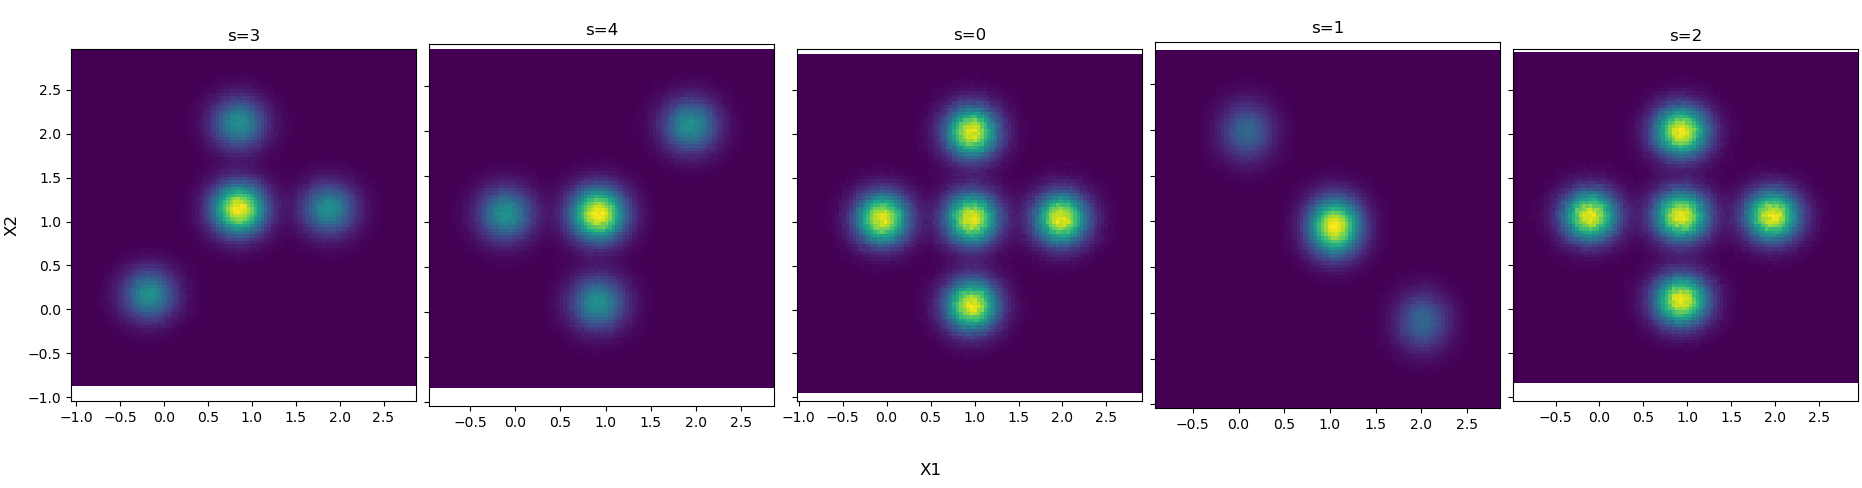
\includegraphics[width=12.0cm]{figures/5_dist_sum.png}
	\vspace*{0.3cm}
	\caption{2-share leakage distributions over $\mathbb{Z}_5$, uniform sensitive variable.}\label{fig:dist5_sum}\vspace*{-0.0cm}
\end{figure}

Intuitively, XOR operation acts independently for each bit, leads to a certain \fxnote[]{wording} relations among operands' HWs (e.g. $\text{HW}(X\oplus Y) = \text{HW}(X) + \text{HW}(Y) - 2\cdot\text{HW}(X\times Y)$), hence, produces well-separate distribution shapes for each value. The arithmetic operations (e.g. addition, subtraction, modulo) let results from lower-order bits affect higher-order bits through the carry (or borrow) bits, leads to more unclear connection.In addition, because it is frequently applied at the end, the binary representation of the moduli has a significant impact on the variety of the distribution shapes.
\todo{Add more info on dist of diff prime in A?}

If $S$ is uniform over $\mathbb{Z}_Q$ there should not be much different between representations, for example, in Fig.\ref{fig:dist5}, \ref{fig:dist11}, we can see even they look different in shapes but generally they have the same number of shapes.
 
However, when we take the small support of $S$ into account, the dissimilarity of these distributions generated by different encoding representation emerges clearly. In  Fig.\ref{fig:dist}, there certainly is a significant different between two representations. It is reasonable to question the gap of the amount of information about sensitive variable $S$ given these two sets of distributions.
\begin{figure}
	\centering 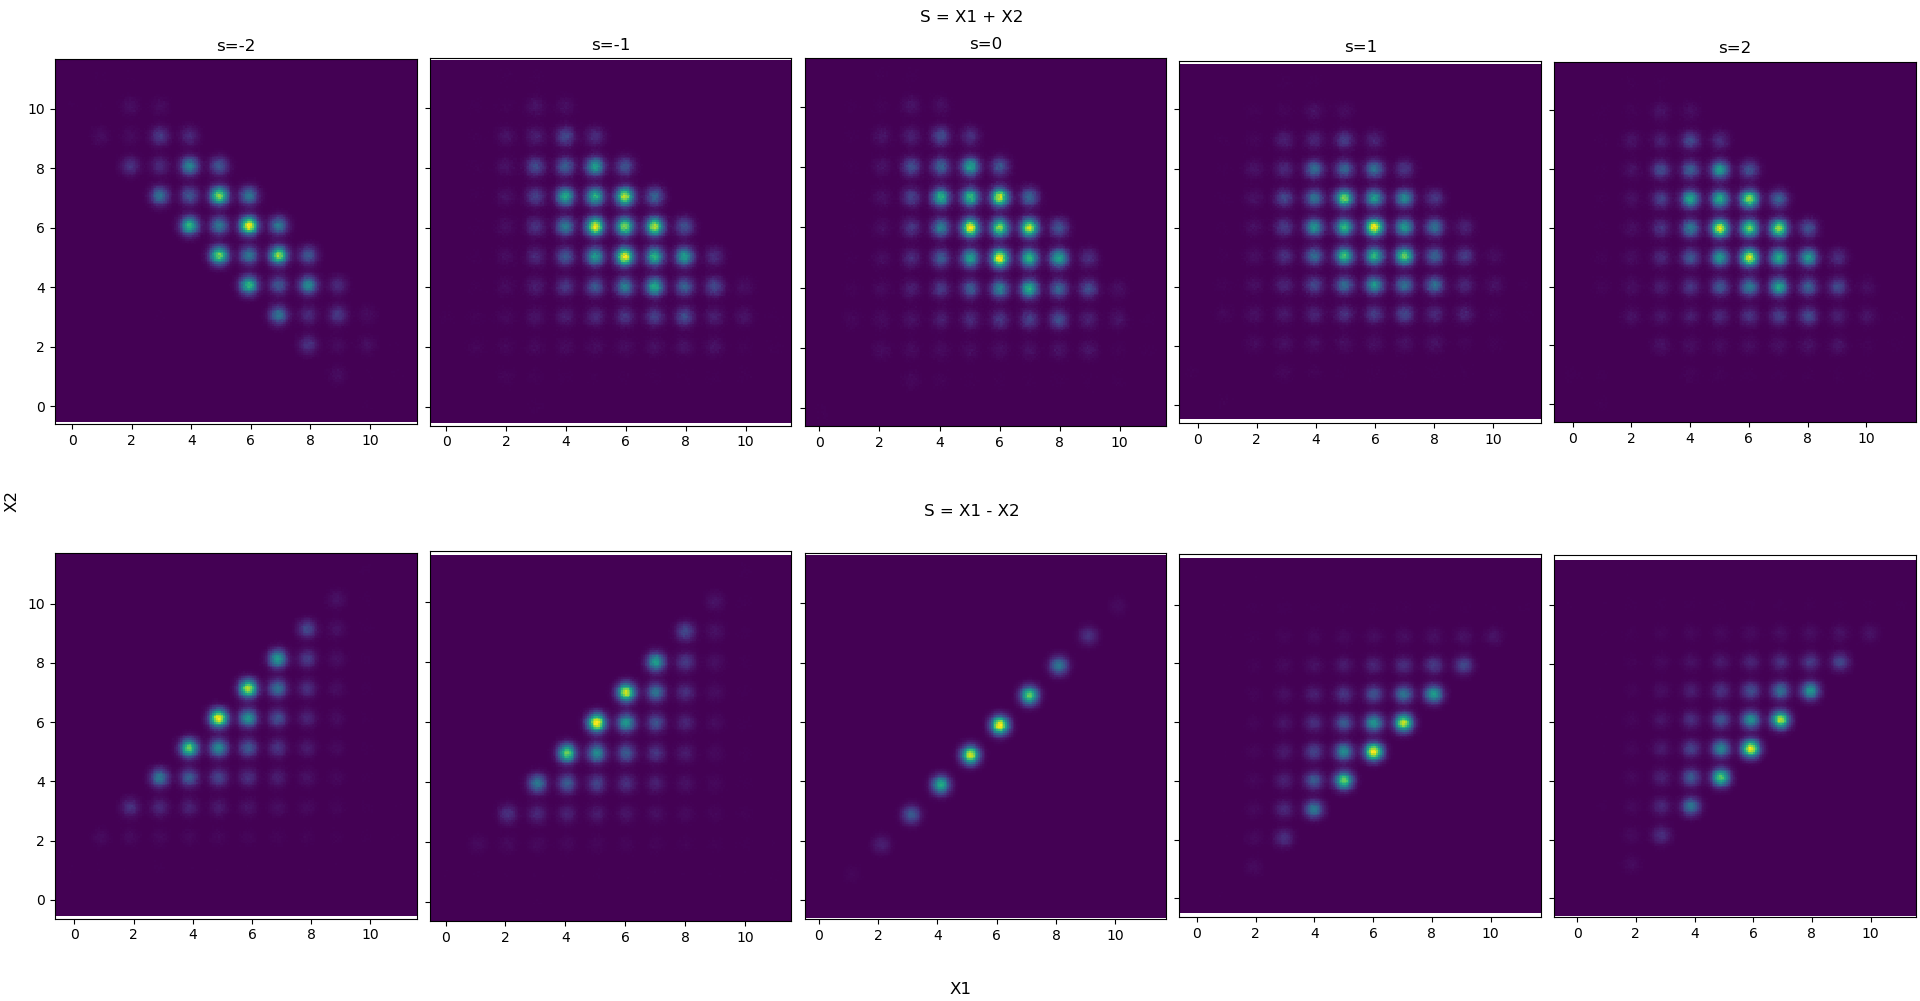
\includegraphics[scale=0.25]{figures/3329_dist_modes.png}
	\caption{2-share leakage distributions over $\mathbb{Z}_Q$.}\label{fig:dist}\vspace*{-0.0cm}
\end{figure}

\subsection{Quantify observations}
We next evaluate concretely the information exposed from the leakages of different encoding representations by its MI with the sensitive variable $S$. With $f(li|xi)$ described in Eq.\ref{eq:gl}, we first compute $p(x_i|l_i)$ followed Bayes theorem as in Eq.\ref{eq:f2p}, we, then, obtain $p(s|\bm{l})$ from SASCA. We let $d$ runs from 2 to 6 and $\sigma^2$ runs from $10^{-3}$ to $10^2$, the results are shown in Fig.\ref{fig:mi234}.
\begin{figure}[h]
	
	\begin{subfigure}{0.5\textwidth}
		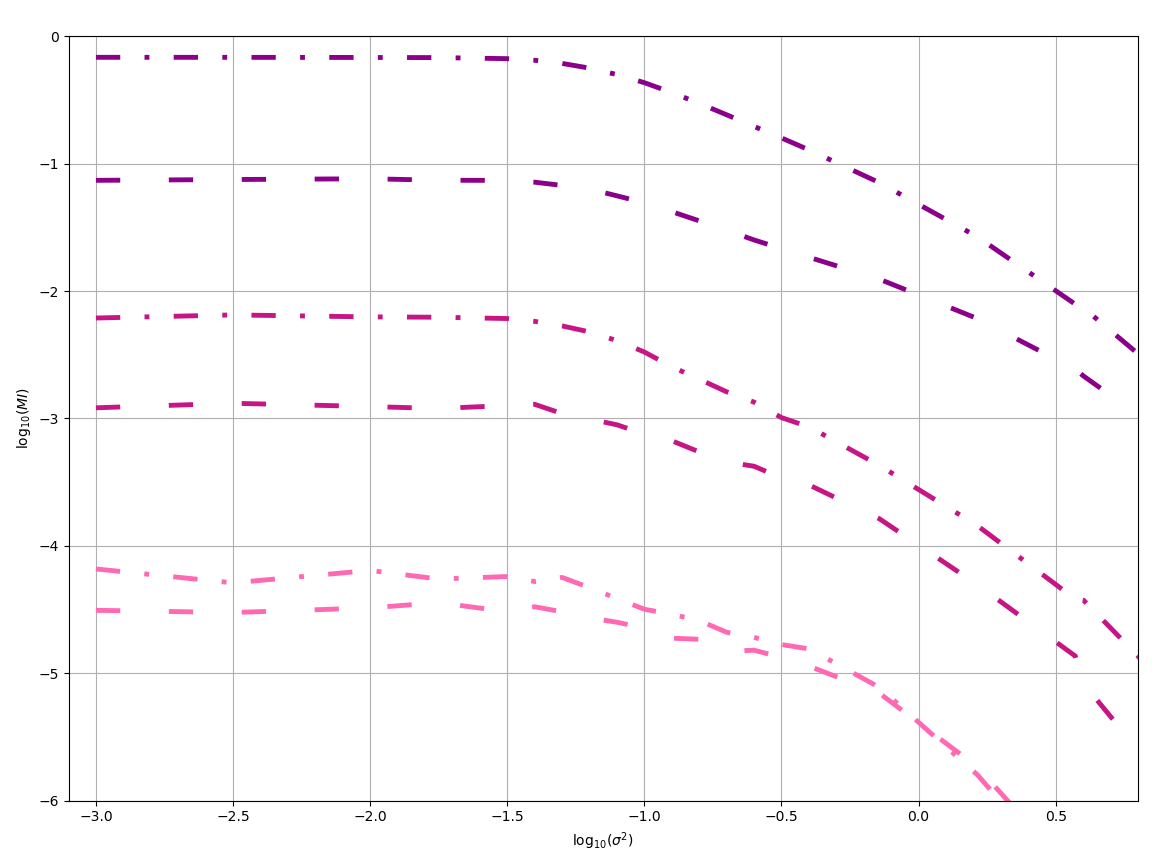
\includegraphics[scale=0.14]{figures/mi_234.png} 
		\caption{MI on simulated data $d$ from  2 to 4 shares, dashed line, dot-dashed lines correspond to $\text{Enc}^{\text{sum}}$, $\text{Enc}^{\text{diff}}$ respectively.}\label{fig:mi234}
	\end{subfigure}
	\begin{subfigure}{0.5\textwidth}
	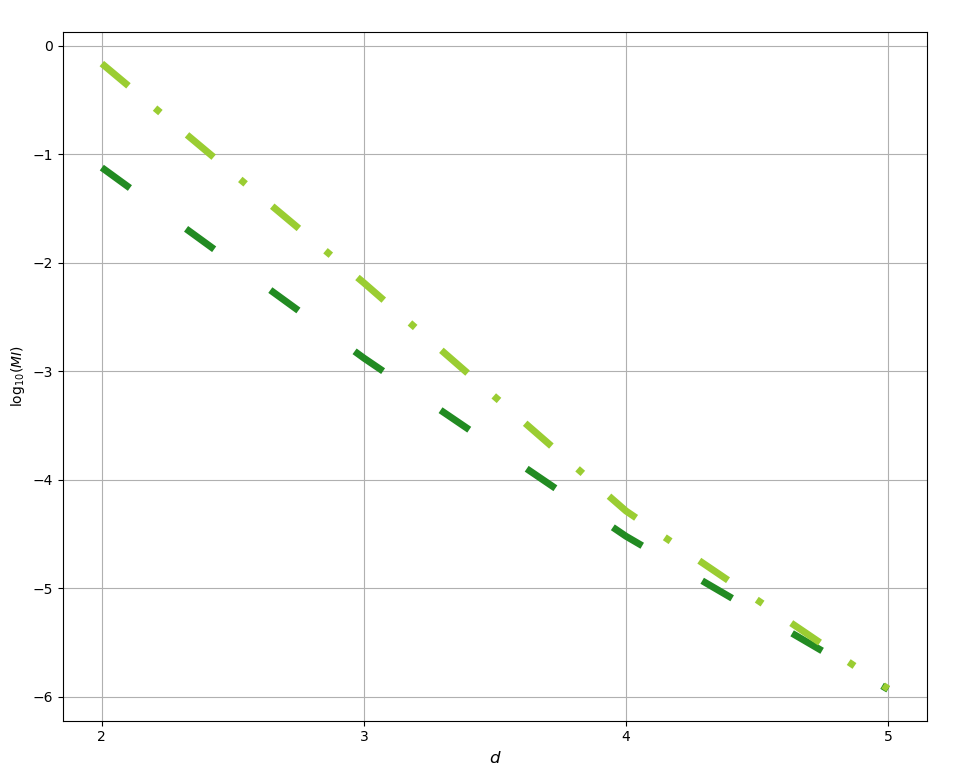
\includegraphics[scale=0.16]{figures/mi_lines_modes.png} 
	\caption{MI on noiseless leakages w.r.t. $d$, dashed line, dot-dashed lines correspond to $\text{Enc}^{\text{sum}}$, $\text{Enc}^{\text{diff}}$ respectively..}\label{fig:milines}
	\end{subfigure}
	\label{fig:image2}
\end{figure}

There are several noticeable observations from this result:
\begin{itemize}
	\item First, we confirm once again noise amplification effect of arithmetic masking in prime-order groups under HW leakage assumption that theoretical hinted in \cite{optimalmask} and experimentally shown in \cite{primemask}. Even when $S$ lies in small set we still have exponential increment of security with respect to number of shares, this trend is stable when noise increases . Additionally, this effect both holds in different encoding representations. 
	\item Next, as anticipated, there is a significant gap between two representations, where leakage from $\text{Enc}^{\text{diff}}$ exposes more information of the secret than $\text{Enc}^{\text{sum}}$. This gap is a factor of ten for $d=2$ and seems to decreases when the number of shares increases.
\end{itemize}
We would like to stress the notable gap between two representations. There would be no difference to mask $S$ as $\text{Enc}^{\text{diff}}$  or $\text{Enc}^{\text{sum}}$  if $S$ is uniformly distributed over $\mathbb{Z}_Q$ \todo{Show this in A?}. However, when $S$ only take few specific values, operations on shares matter. For example, in 2-share case, $s=0$ is exposed totally given $\text{HW}(X_1)$ and $\text{HW}(X_2)$ in  $\text{Enc}^{\text{sum}}$ but there is no such value of $s$ in $\mathcal{S}$ has the same issue if $\text{Enc}^{\text{diff}}$ is used(this could be viewed as an homomorphic attack" as suggested in \cite{optimalmask}).

Additionally, the difference between two ways of encoding diminishes when number of shares $d$ increases. We confirm this trend with smaller prime-order group $\mathbb{Z}_{23}$(Fig.\ref{fig:miq23})\todo{Better fig}. We adopt the reduction to random walks as \cite{optimalmask} then the length of operation repetition seems to be relevant. For example, in considering $d=4$, we have $S^\text{diff} = X_1 + X_2 + X_3 + X_4$ in $\text{Enc}^{\text{diff}}$  and $S^\text{sum} = -X_1 - X_2 - X_3 + X_4$   in $\text{Enc}^{\text{sum}}$ then intuitively, $Z_1 + Z_2 + Z_3 + Z_4$ is close to uniform than $-Z_1 - Z_2 - Z_3 + Z_4$. By trying two other representations:
\begin{align*}
	S^1 &= -X_1 + X_2 + X_3 + X_4\\
	S^2 &= -X_1 - X_2 + X_3 + X4,
\end{align*}
and compute MI corresponds to each one in the same manner, we obtain results depicted in Fig.\ref{fig:mi_4shares}.
\begin{figure}[h]
	\vspace*{-0.0cm}
	\hspace*{0.0cm}\centering 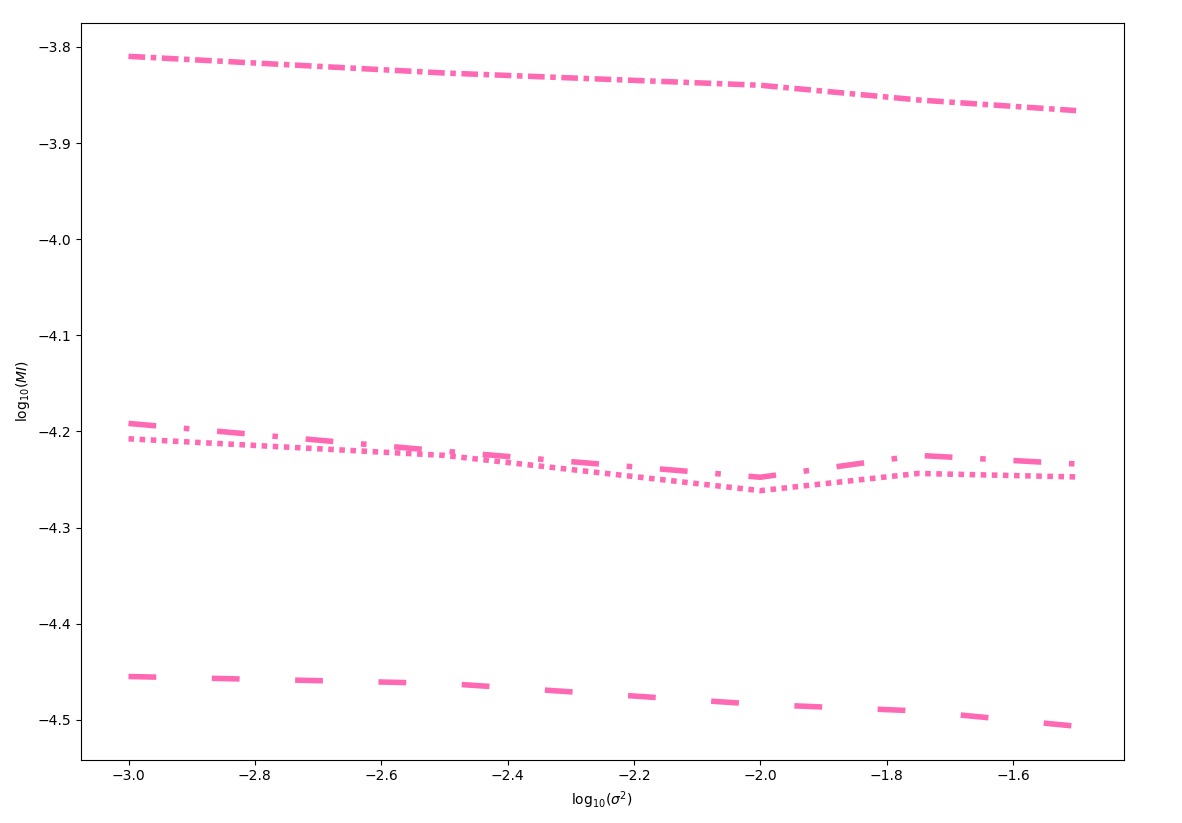
\includegraphics[scale=0.2]{figures/4shares_modes.png}
	\vspace*{0.3cm}
	\caption{MI for 4 different representations for 4-share encoding.}\label{fig:mi_4shares}\vspace*{-0.0cm}
\end{figure}
\todo{Better fig}

It somehow infers the impact of operation repetition as suspected. Where this length is equal and is 3 in $S^\text{sum}$ and $S^1 $, we gain the same amount of information about $S$ given $\bm{L}$. We have the least in $S^\text{diff}$ where this length is the longest (i.e., 4) and have the most information in $S^2$ where this length is 2.

We emphasize that this interpretation is merely experimental and lacks of concrete theoretical proof. However, we are certain that this trend can be explained in formal manner.
\section{Real-world analysis}\label{sec:onm}
We next put the observations in simulation to test with real measurements.

We note that several available polynomial masking for KYBER \cite{Kmaskimp0},\cite{Kmaskimp1}, \cite{Kmaskimp2} and all polynomial masking schemes for KYBER (especially and for PQC in general) such as \cite{Kmask1} \fxnote[]{more citations} use $\text{Enc}^{\text{diff}}$ for their representation. This is positive sign as it has been shown in simulation that it allows exponential security with respect to the number of shares $d$ and $\text{Enc}^{\text{diff}}$ provide better security compare to $\text{Enc}^{\text{sum}}$. However, depending on the implementation, the leakage can actually be in form of $\text{Enc}^{\text{sum}}$. Normally to mask a coefficient of the secret $s$, the computations follow:
\begin{enumerate}
	\item Copy $s$ to the last (or the first) share $x_d \leftarrow s$.
	\item Generate a random number $r$ in $\mathbb{Z}_Q$.
	\item Assigning the shares and accumulating the them can be done in two ways:
	\begin{itemize}
		\item Assign $x_i \leftarrow r$ and accumulate on the last share $x_d = x_d - r$, or
		\item Assign $x_i \leftarrow Q - r$ and $x_d = x_d + r$.
	\end{itemize}
\end{enumerate}
Both ways in step 3 eventually leads to $\text{Enc}^{\text{diff}}$ representation but notice if we have that leakage corresponding to $r$ then the second ways of computing share gives us the leakage corresponding to $\text{Enc}^{\text{sum}}$.

We then use the same implementation such as \cite{Kmaskimp0} but use leakage on $x_i$ and $x_d$ to produce data for $\text{Enc}^{\text{diff}}$ and use leakage on $r$ and $x_d$ to produce data for $\text{Enc}^{\text{sum}}$.

We run our implementations on Arm Cortex-M4 STM32F415 and acquire two million traces for each implementation. We first compute SNR on the data to make sure there is no first-order information of $S$ in the traces and to select relevant PoIs for the next step\footnote{SNR on traces are shown in Fig.\ref{fig:snr2}}. In order to compare between implementations, we again, base on IT metric, and PI to be more specific.

We proceed our evaluation in several steps:
\begin{enumerate}
	\item For each share, we select $n_{\text{PoI}}$ points in the traces that have maximum SNR correspond to that share. We then have truncated leakage $\bm{L}'_i$ for each share. These shares' leakages are then concatenated to be reduced traces $\bm{L}'$ or kept separately depends on the distinguisher in use.
	\item We then use $\bm{L}'$ or $\bm{L}'_i$ to model $p(s|\bm{l}')$ directly or $p(x_i|\bm{l}'_i)$. In the latter case, we combine $p(x_i|\bm{l}'_i)$ to obtain $p(s|\bm{l}')$ eventually.
	\item PI is estimated using Eq.\ref{eq:pi} on the model given by the previous step.
\end{enumerate}

We use different distiguishers to model the unknown $p(\cdot|\cdot)$ to inspect the leakages in different assumptions. 
The distiguishers are:
\begin{description}
	\item[Plain MLP] We feed MLP the reduced traces $\bm{L}'$ and use it to directly model $p_(s|\bm{l})$ and PI is estimated based on MLP's output. The model $p_(s|\bm{l})$ is estimated without any assumption about the leakage. We make sure that the selected points do not have maximal SNR value w.r.t. the secret to avoid any first-order information of the secret.
	\item[MLP x SASCA] We keep truncated traces for each share $\bm{L}'_i$ separately. Then we use MLP to model $p(x_i|\bm{l}_i)$ for each share. The results then are fed to SASCA to obtain $p(s|\bm{l})$. We restrict the information of the secret is only from the leakage of its shares, however, there is no assumption on the shares' leakage.
	\item[LDA x SASCA] Similar process as MLPxSASCA, we used truncated traces $\bm{L}'_i$  to build the model for $p(x_i|\bm{l}_i)$ separately using LDA. In LDA, the truncated traces  $\bm{L}'_i$  are projected to subspace of dimension $n_{\text{LDA}}$, then GMT are applied as described in Sec.\ref{ssec:lda} to obtain  $p(x_i|\bm{l}_i)$. Finally, $p(s|\bm{l})$ is estimated using SASCA. In this setting, shares' leakages are assumed to be multivariate Gaussian distributed and satisfy homoscedasticity.
\end{description}
\todo{Optimal  $n_{\text{PoI}}$ , optimal $n_{\text{LDA}}$}
We compare convergence rates among distiguishers by compute PI correspondingly to increasing number of profiling traces $N_p$. The results is shown in Fig.\ref{fig:pi}.\todo{Complete this fig}
\begin{figure}[h]
	\vspace*{-0.0cm}
	\hspace*{0.0cm}\centering 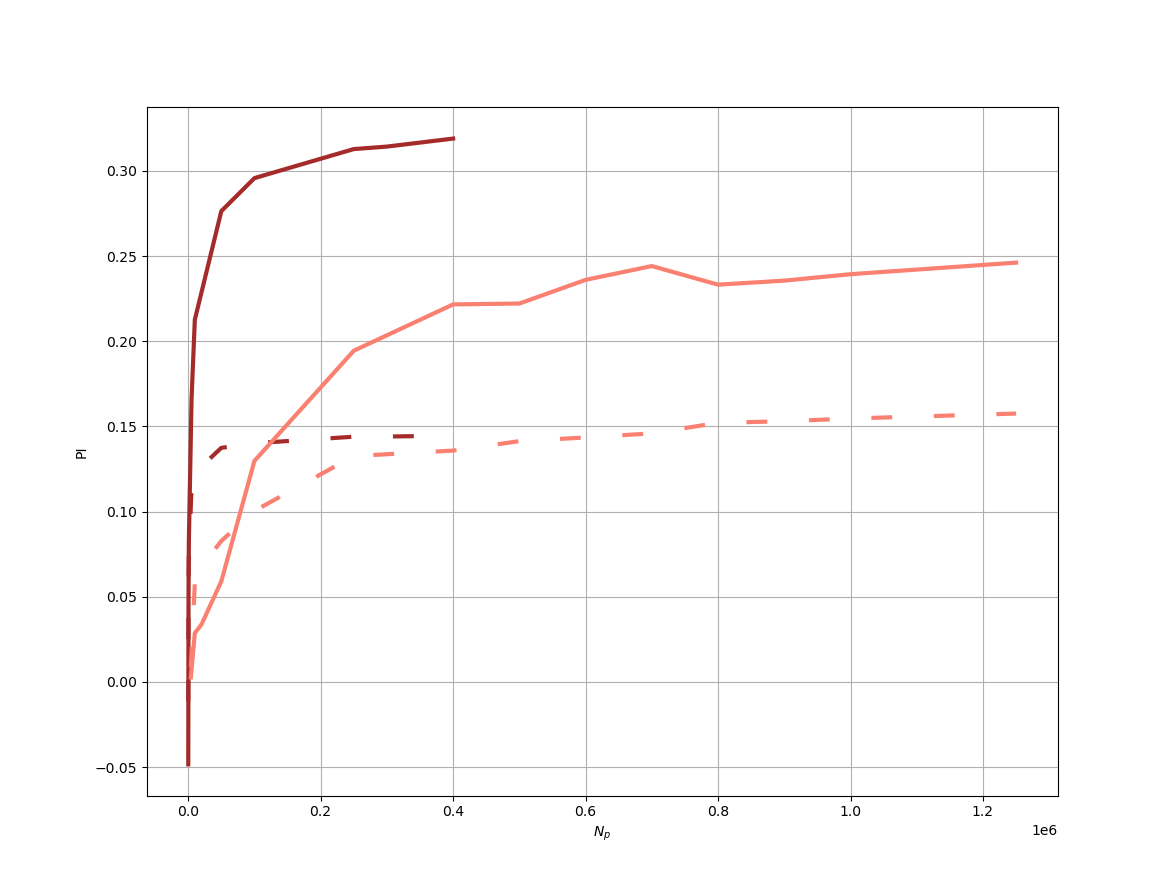
\includegraphics[scale=0.3]{figures/pi_mlps.png}
	\vspace*{0.3cm}
	\caption{PI of different distinguishers. Brown and salmon curves correspond to Plain MLP and MLPxSASCA, solid and dashed curves correspond to $\text{Enc}^{\text{diff}}$ and $\text{Enc}^{\text{sum}}$  respectively.}
	\label{fig:pi}
\end{figure}
\section{Conclusion}
\appendix
\section{Supplementary}
\begin{figure}
	\centering
	\begin{subfigure}{1\linewidth}
		\centering
		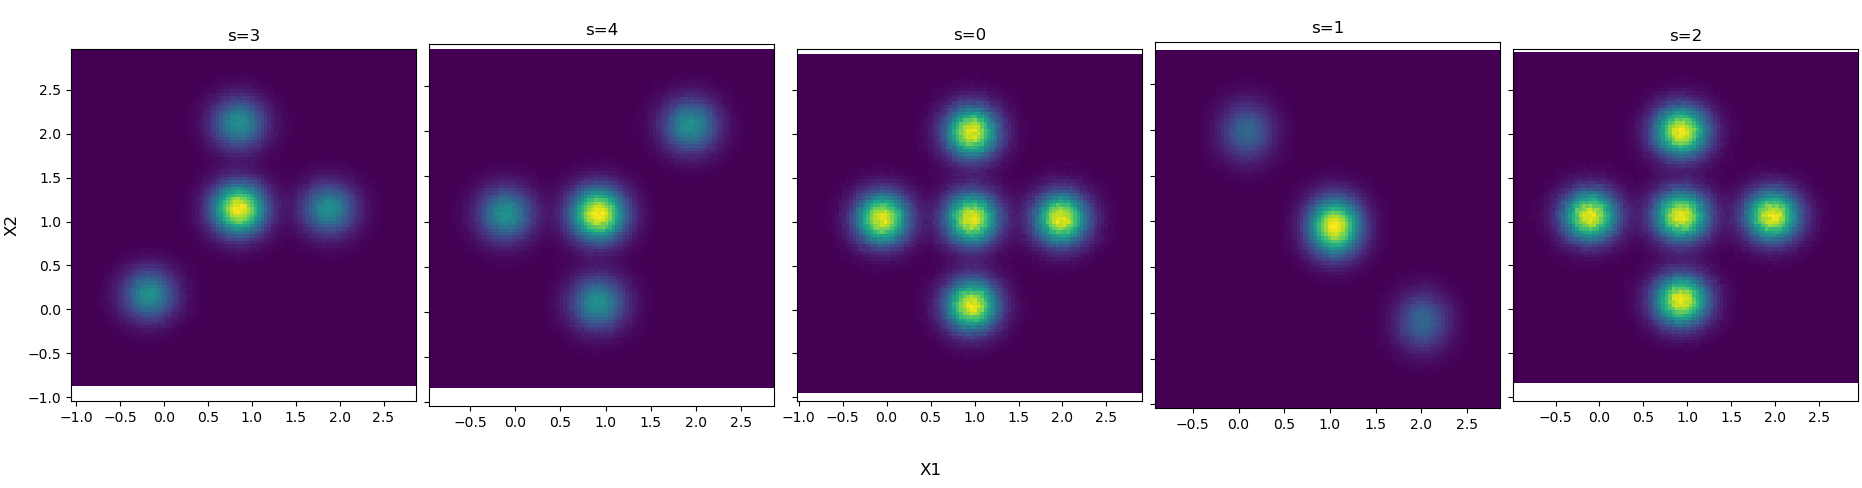
\includegraphics[scale=0.2]{figures/5_dist_sum.png}
	\end{subfigure} %
	
	\hfill
	
	\begin{subfigure}{1\linewidth}
		%\centering
		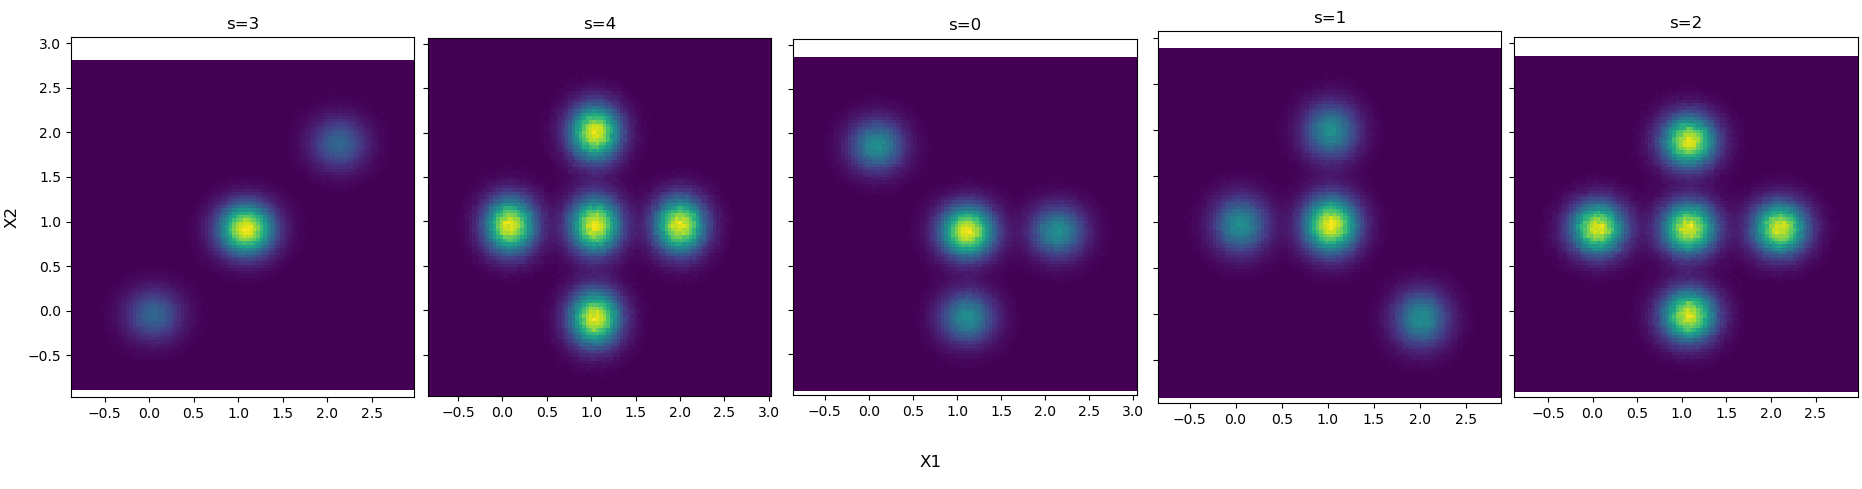
\includegraphics[scale=0.2]{figures/5_dist_diff.png}
	\end{subfigure}
	\caption{Leakages distribution for uniform secret over $\mathbb{Z}_5$. Top and bottom figure is corresponding to  $\text{Enc}^{\text{sum}}$ and  $\text{Enc}^{\text{diff}}$ respectively}
	\label{fig:dist5}
\end{figure}

\begin{figure}
	\centering
	\begin{subfigure}{1\linewidth}
		\centering
		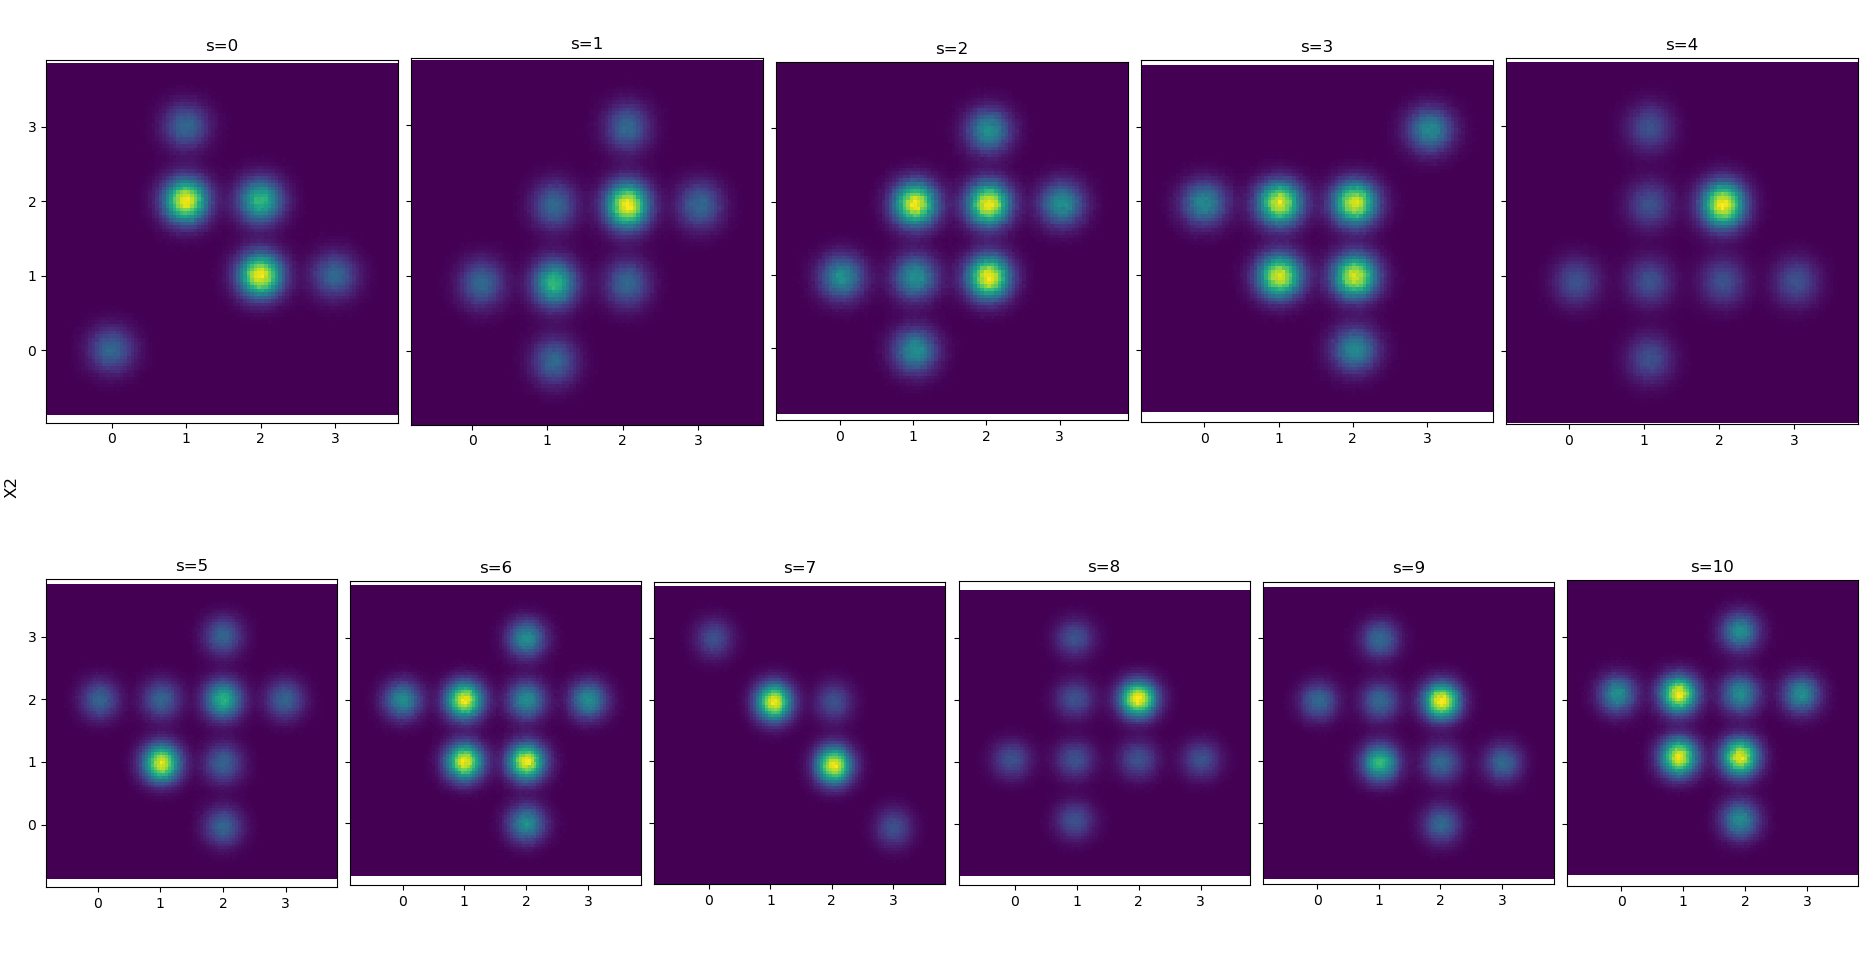
\includegraphics[scale=0.25]{figures/11_dist_sum.png}
		\caption{Leakages distribution of $\text{Enc}^{\text{sum}}$ }
		\label{fig:dist11_sum}
	\end{subfigure} %
	
	\hfill
	
	\begin{subfigure}{1\linewidth}
		%\centering
		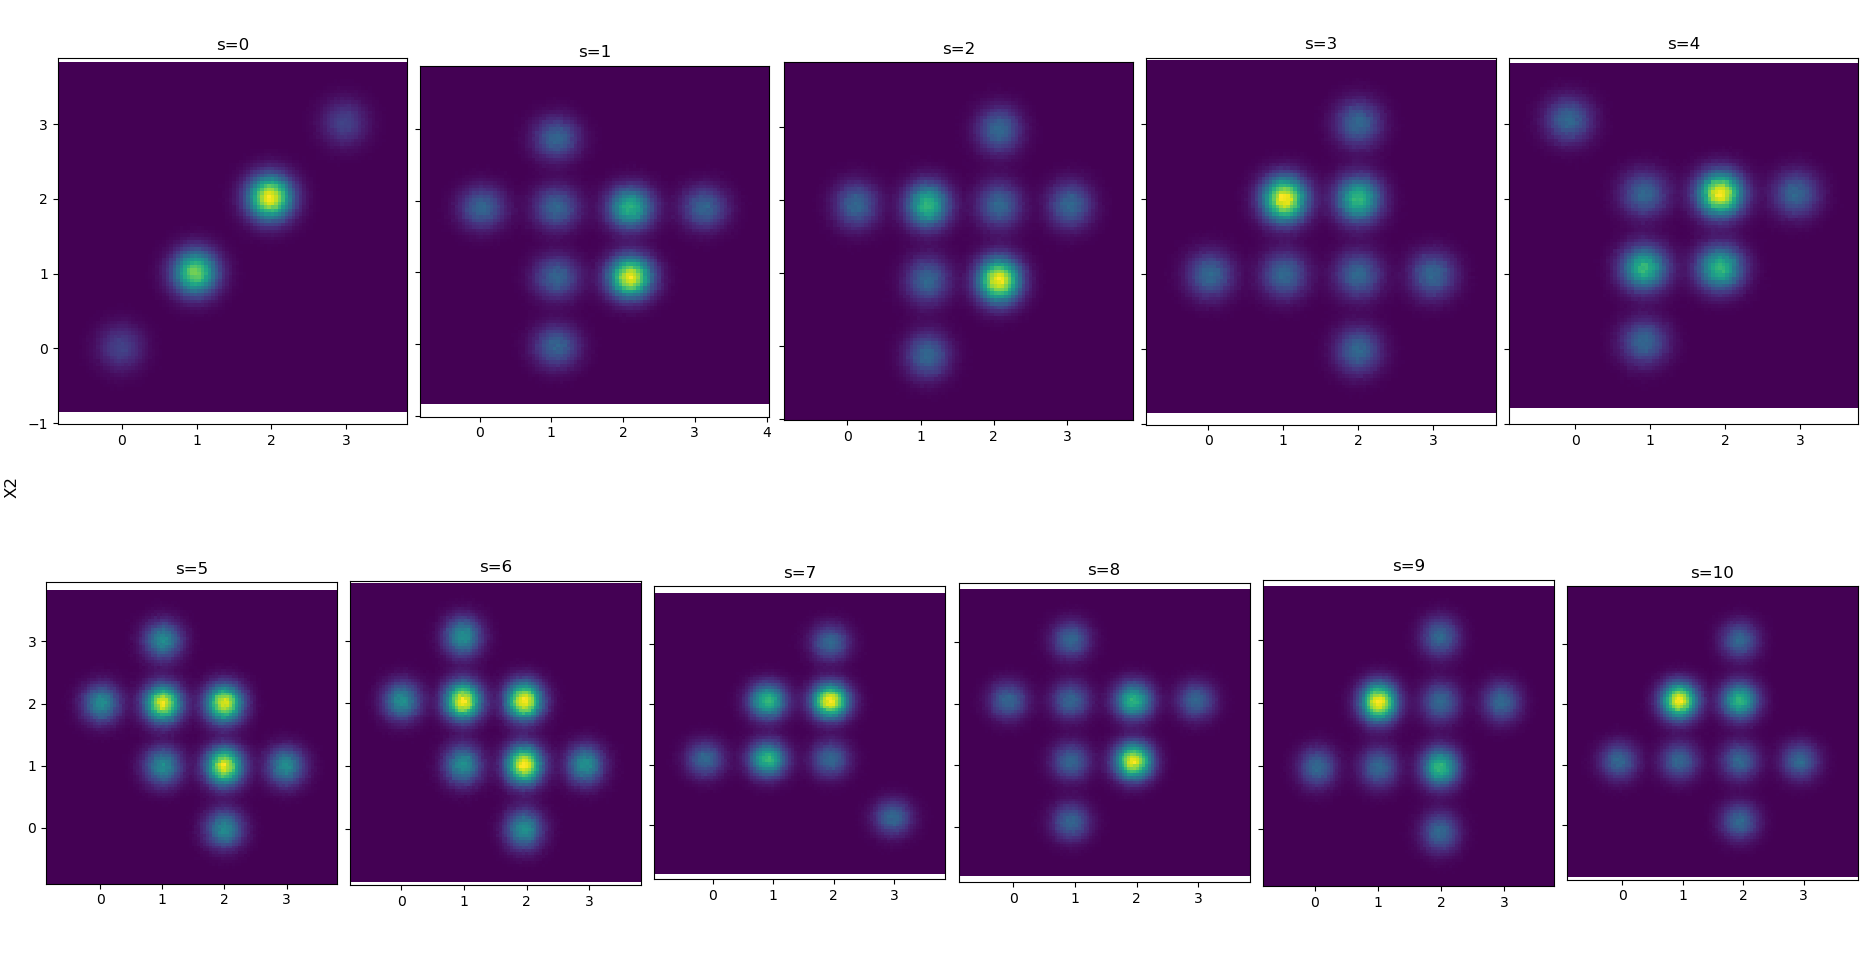
\includegraphics[scale=0.25]{figures/11_dist_diff.png}
		\caption{Leakages distribution of $\text{Enc}^{\text{diff}}$ }
		\label{fig:dist11_diff}
	\end{subfigure}
	\caption{Leakages distribution for uniform secret over $\mathbb{Z}_{11}$, Fig.\ref{fig:dist11_sum} , Fig.\ref{fig:dist11_diff} corresponds to $\text{Enc}^{\text{sum}}$, $\text{Enc}^{\text{diff}}$ respectively.}
	\label{fig:dist11}
\end{figure}


\begin{figure}
	\vspace*{-0.0cm}
	\hspace*{0.0cm}\centering 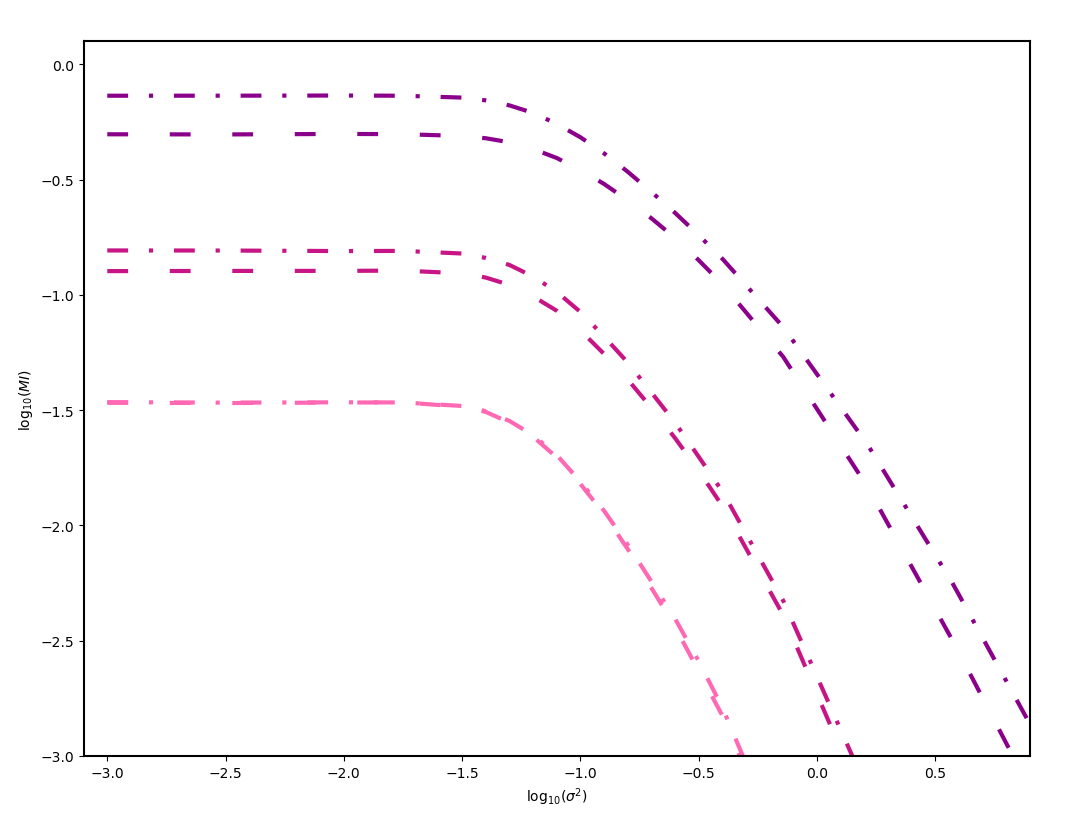
\includegraphics[width=12.0cm]{figures/MI_23_234.png}
	\vspace*{0.3cm}
	\caption{SNR on traces, top figures correspond to $\text{Enc}^{\text{sum}}$, bottom figures correspond to $\text{Enc}^{\text{diff}}$, left figures are SNR on shares where blue and orange line correspond to the first and second share respectively, right figures are SNR on secret.}\label{fig:miq23}\vspace*{-0.0cm}
\end{figure}
\begin{figure}
	\vspace*{-0.0cm}
	\hspace*{0.0cm}\centering 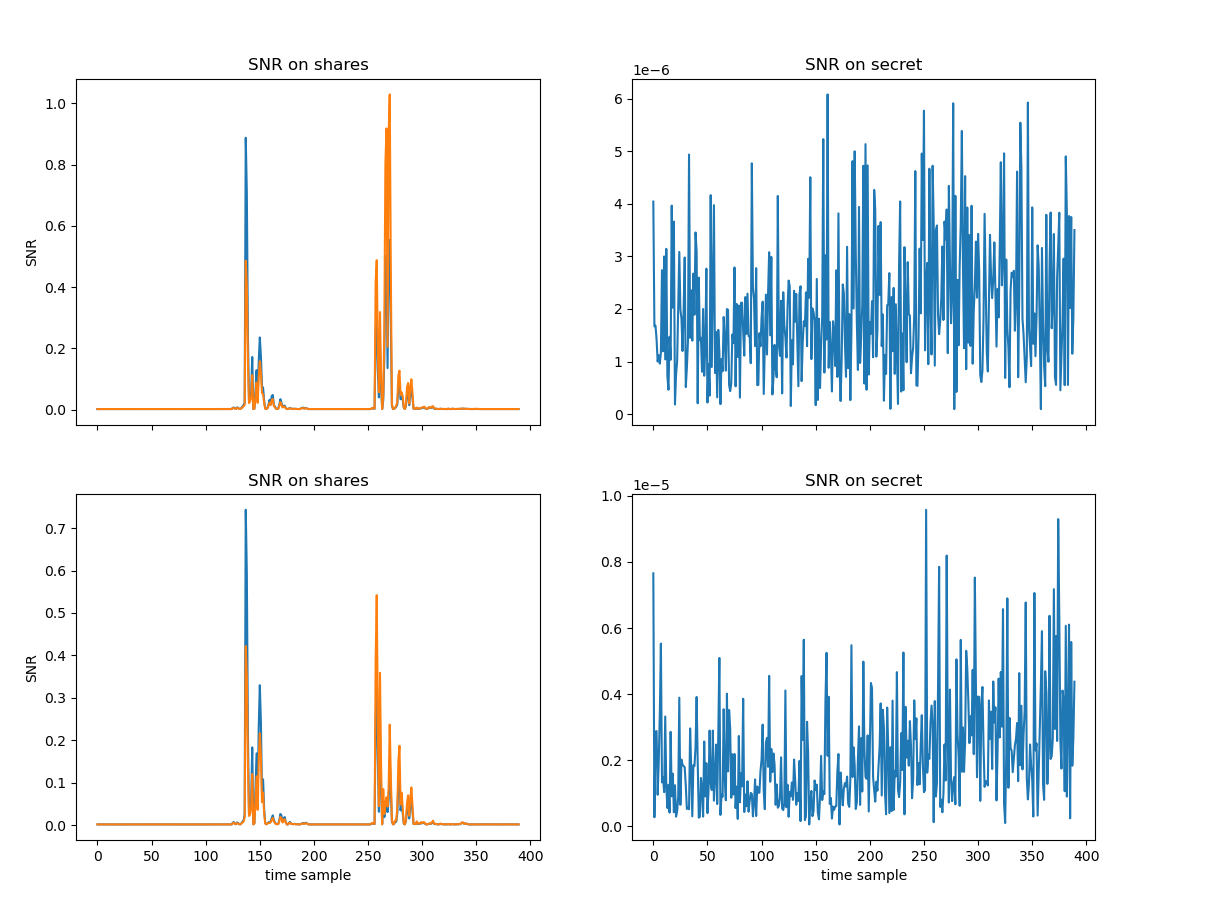
\includegraphics[width=12.0cm]{figures/snr_2shares.png}
	\vspace*{0.3cm}
	\caption{SNR on traces, top figures correspond to $\text{Enc}^{\text{sum}}$, bottom figures correspond to $\text{Enc}^{\text{diff}}$, left figures are SNR on shares where blue and orange line correspond to the first and second share respectively, right figures are SNR on secret.}\label{fig:snr2}\vspace*{-0.0cm}
\end{figure}
\bibliographystyle{alpha}
\bibliography{refs}

\end{document}
